% !TEX root=../../thesis.tex

\section{Stakeholders} % (fold)
\label{sec:back_stakeholders}
When looking at the Norwegian railway, there exists several types of users which
may be taken into consideration. On the Norwegian railway operates several
companies, who all have several positions in their organization hierarchy. Each
of these positions have different responsibilities and therefor different
interests in the system. A example of such a hierarchy is presented in
\Ref{table:user_roles}.

\begin{table}[!h]\small
	\begin{tabularx}{\textwidth}{|l|X|}
		\hline
		User type & Responsibility \\
		\hline
		Railway director & Organization director\\
		\hline
		Infrastructure director & Responsibility to facilitate that the railway traffic in Norway is safe and reliable\\
		\hline
		Area director & Responsible for an area\\
		\hline
		Stretch director & Responsible for a stretch\\
		\hline
		Segment director & Responsible for a segment\\
		\hline
	\end{tabularx}
\caption{User roles in the Norwegian railway network}
\label{table:user_roles}
\end{table}

The hierarchy presented in the table is based on the organization structure of
Jernbaneverket shown in \Ref{fig:jbv_infrastructure_org_map}. As stated in
\Ref{sec:railway_operations}, these stakeholders/divisions need to cooperate 
in order to provide safety and punctuality, both within the company and 
between the infrastructure owner and undertakings. Since the different 
stakeholders have different responsibilities but need to cooperate, they have 
concerns which overlap. 

An examples of stakeholders concerns overlapping can 
be taken from the example presented in \Ref{sec:railway_operations}. The 
material division is concerned with the maintainability of the material; the 
planning division is concerned with the capacity presented from the 
infrastructure owner, demands from the passengers; the passenger trains east/
region divisions is concerned with the personnel; the traffic division is
concerned that the traffic is executed according to schedule. 

In the infrastructure divisions, the traffic- and marketing division is
concerned with planning of the schedule; the infrastructure division is
concerned with errors, and accounts for many of the speed restrictions, while
they are partly under the responsibility of the security staff.\\


During the work of this thesis, we use parts of the hierarchy presented in 
\Ref{table:user_roles} based on the organizational structure of Jernbaneverket.
\begin{description}
	\item [Area director] - Responsible for one of six areas in which the 
	Norwegian railway is divided into.
	\item [Stretch director] - Responsible for one of several stretches within 
	one area.
	\item [Segment director] - Responsible for a segment of stations within one stretch.
\end{description}

\bigskip\bigskip\bigskip
An example of such a hierarchy is presented in the list below.

\begin{description}
	\item [Area] - Midt (Middle-part of Norway).
	\item [Dovre- og Raumabanen] - The northern part of the Dovreline and the
	Rauma line.
	\item [(Dombås) - Hjerkinn] - The segment of the Dovreline which is 
	between the exit of the station on Dombås and the entrance to Hjerkinn
	station.
\end{description}

% section stakeholders (end)

\section{Datasets} % (fold)
\label{sec:back_data_sets}
There are much data to process when performing a study of a relatively complex 
system as the Norwegian railway, as the different information types are stored
independently.\\

As Hegglund\cite[pp. 10-11]{hegglundPunklighetsdataIJernbanetraffik} describes,
Jernbaneverket measures punctuality data in two different ways and stores the
data in a punctuality database called TIOS, \Ref{fig:jernbaneverket-trafikkdata} shows a extract from the TIOS database. They either have automatic measurements of when a 
trains passes a measure point on the eastern part of Norway, or manual 
registration in the rest of the country of each passing. In 2012,  884 passenger trains passed Oslo central station alone per day \cite[p. 12]{jernbaneverketStatistikk}.
Since the passing of a measurement point by a train is being stored, large sets
of data gets accumulated over time.

\begin{figure}[!htbp]
	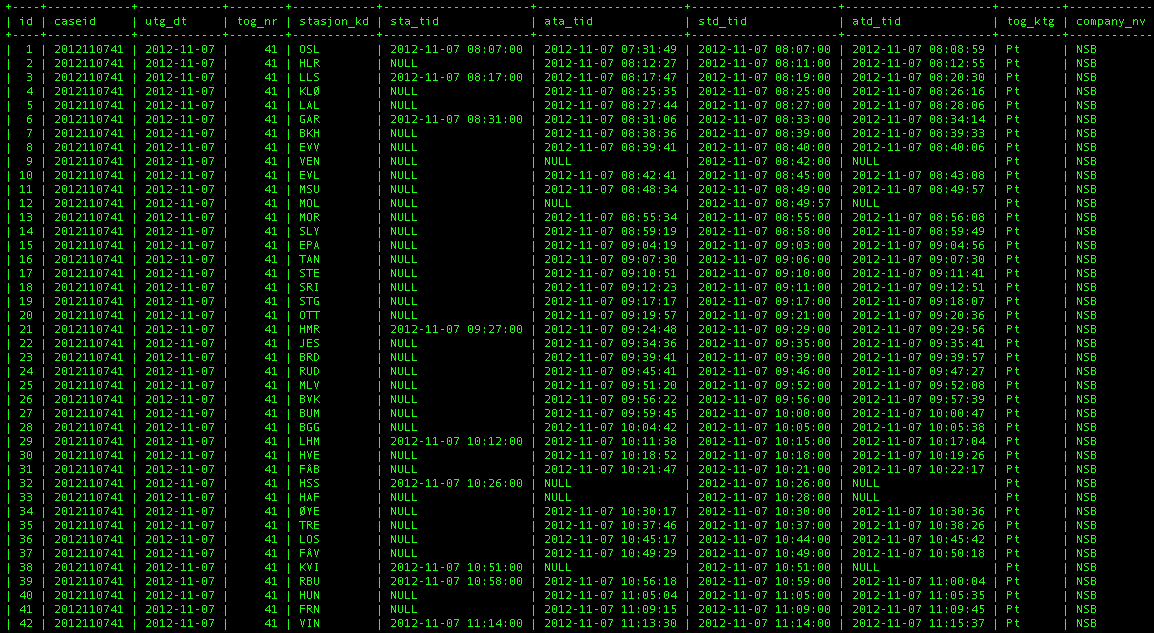
\includegraphics[width=\textwidth,center]{trafikkdata.png}
	\caption[TIOS Punctuality data]{TIOS Punctuality data \cite{sintefPresis}}
	\label{fig:jernbaneverket-trafikkdata}
\end{figure}

Since the set of data stored in TIOS, stores every train that passes every 
measurement point, and the corresponding time point , is is possible
to use the same set to calculate where every crossing between different trains
happens. The usage of the same set is possible since one can compare the time 
stamps of the passing of each station to another train.\\

When the speed restrictions are registered, they are stored in their own set of
data which is based on the users filling out different forms. The speed
restriction sets are based on forms filled out by users, and cover both
scheduled work and unscheduled work. Examples of scheduled work can be
improvement on infrastructure, and example of unscheduled work can be destroyed
tracks due to flooding. \\

Analyzing large different sets of data which might originate from different
sources, will be required when a method shall be aware of the stakeholder.
When developing such a method, one also needs to have a good way of limiting
the visual representation of the data to avoid filling the display with to much
information.
% section data_sets (end)

\section{Aggregation} % (fold)
\label{sec:back_aggregation}

When using the hierarchy of relevant stakeholders presented in \Ref{sec:back_stakeholders}
and the large sets of data mentioned in \Ref{sec:back_data_sets}, a
good way to limit the amount of data presented is to aggregate over the sets of
data based on hierarchy.

If one look at the example hierarchy presented in Section
\Ref{sec:back_stakeholders}, an example of such an aggregation is as
follows. The segment director wants information of every station along the
segment. The Stretch director wants summarized information from each segment, which is
aggregated from the stations. The area director wants information of every
stretch, which is aggregated from each segment.

When one is aware of the different level of details each type of stakeholder
wants, the aggregation quickly becomes a useful way of determining the
necessary data.

% section aggregation (end)
